\documentclass{article}

\usepackage[final]{style}
\usepackage[utf8]{inputenc} % allow utf-8 input
\usepackage[T1]{fontenc}    % use 8-bit T1 fonts
\usepackage{hyperref}       % hyperlinks
\usepackage{url}            % simple URL typesetting
\usepackage{booktabs}       % professional-quality tables
\usepackage{amsfonts}       % blackboard math symbols
\usepackage{nicefrac}       % compact symbols for 1/2, etc.
\usepackage{microtype}      % microtypography
\usepackage{verbatim}
\usepackage{graphicx}       % for figures
\usepackage[]{algorithm2e}


\title{Lecture \#19: Introduction to Deep Learning}

\author{
  Vineet Edupuganti, Mihir Garimella, Ben Kotopka, Prathik Naidu, Rohan Suri \\
  Department of Computer Science\\
  Stanford University\\
  Stanford, CA 94305 \\
  \texttt{\{ve5, mihirg, bkotopka, prathik.naidu, rsuri2\}@cs.stanford.edu} \\
}

\begin{document}

\maketitle

\section{Introduction}
So far in this class, we've covered a wide range of classical computer vision techniques, including edge detection, clustering methods, classifiers, and feature detectors/descriptors. While these  techniques are still highly relevant to computer vision in research and industry, they share one major drawback: they rely on humans to hand-design features and choose classifiers that work well for the specific problem they're trying to solve. As a result, computer vision methods designed to solve one problem are often not readily adaptable to solving other problems, significant human effort and experimentation is required to build reasonably accurate vision pipelines, and even the best-designed pipelines are limited in the accuracy they can achieve simply because they were designed by humans and can therefore only pick up on patterns that human designers have picked up on first.

\textit{Deep learning} is a relatively new method that is now a basic building block of modern computer vision research because it is free from these pitfalls. Instead of relying on hand-selected features and classifiers, deep learning approaches learn how to best digest and interpret data to solve any problem they're trained for. The key to these approaches is that they perform \textit{end-to-end learning}, meaning that they learn how to directly map raw inputs (images in computer vision) to desired output (e.g., labels, segmented images, predictions). Deep learning approaches usually involve combining a small set of simple tools to build a network and then training that network on data for the specific problem you're trying to solve; they can often be adapted to different problems by simply swapping out the training data. Deep learning approaches are very loosely inspired by the brain in that they attempt to mimic neuronal activity in the neocortex of the human brain \cite{hof_2016}.

\section{Applications}
Recently, deep learning has led to rapid progress on several problems in computer vision and related fields. In this section, we will provide a brief overview of progress and current state-of-the-art solutions for a small sampling of these problems.

\subsection{Image Classification}

\textit{Image classification} is the problem of identifying all of the objects present in input images. One common benchmark for this task is performance on the ImageNet dataset \cite{deng2009imagenet}, a large, labeled dataset of 1,431,167 images containing 1,000 different objects (a 50$\times$ increase in the number of objects compared to previous classification datasets).

Initial state-of-the-art algorithms built for the ImageNet challenge were hand-tuned and used a series of carefully-selected, hardcoded features to tokenize test images before feeding this tokenized representation into a classifier, like an SVM, for final classification; for instance, the 2010 state-of-the-art for ImageNet was \cite{lin2011large}, which managed to achieve a 28.2\% top-5 error rate using a pipeline that first computed HOG and LBP descriptors for an image, coded and pooled them together, and then fed them into an SVM. However, so-called "shallow" approaches were quickly beaten by "deep" approaches within the next few years; AlexNet \cite{krizhevsky2012imagenet} in 2012 achieved a 16.4\% error rate with a 8-layer network, VGG \cite{simonyan2014very} in 2014 achieved a 7.3\% error rate with 19 layers, GoogLeNet \cite{szegedy2015going} later that year achieved a 6.7\% error rate with 22 layers, and recently, in 2015, ResNet \cite{he2016deep} achieved a groundbreaking error rate of 3.57\% with 152 layers\textemdash especially impressive considering that the error of a human performing the same classification challenge was only 5.1\% \cite{russakovsky2015imagenet}.

In general, this pattern indicates an exciting for the future of deep learning algorithms in computer vision; deep learning algorithms can rapidly outperform classical computer vision techniques\textemdash and even, in some sense, outperform humans\textemdash for very nuanced, difficult vision tasks, especially as the number of layers and network complexity is scaled up.

\subsection{Object Detection}

\textit{Object detection} is an extension of the image classification task that aims to not only answer the question "what?" (i.e., recognize the objects in the image) but also answer the question "where?" (i.e., localize the recognized objects). Before deep convolutional neural networks (see Section 6 for more information on what these actually are), the mAP of "shallow" computer vision approaches on the PASCAL VOC dataset \cite{everingham2015pascal} flattened out at around 40\% in 2012, breaking the trend of continuous accuracy improvements in prior years and indicating that shallow approaches couldn't do much better for this task. However, deep learning approaches were able to increase this accuracy to around 52\% just the next year, in 2013, and have been continuously demonstrating a rapid upward accuracy growth trend up to the current state-of-the-art performance for this task, an impressive 85.6\% mAP from \cite{he2016deep}.

\subsection{Object Segmentation}

\textit{Object segmentation} involves first dividing an object into different semantic regions, usually representing different objects, and then determining what type of object each region contains. This is especially challenging to do generically with classical segmentation algorithms like the ones we learned in class\textemdash we need specific knowledge of the objects we're interested in detecting, and then must hand-design features tailored to each object using this prior knowledge (e.g., we know that donuts are circular with holes in the middle, so we design a feature that prioritizes these sorts of shapes). However, recent deep learning approaches have demonstrated impressive results to solving this difficult task of first segmenting an image and then identifying each object without having humans encode intuition about a small set of objects to look for; for example, \cite{semseg} uses three separate deep networks to achieve the results shown below.


\begin{figure}[b]
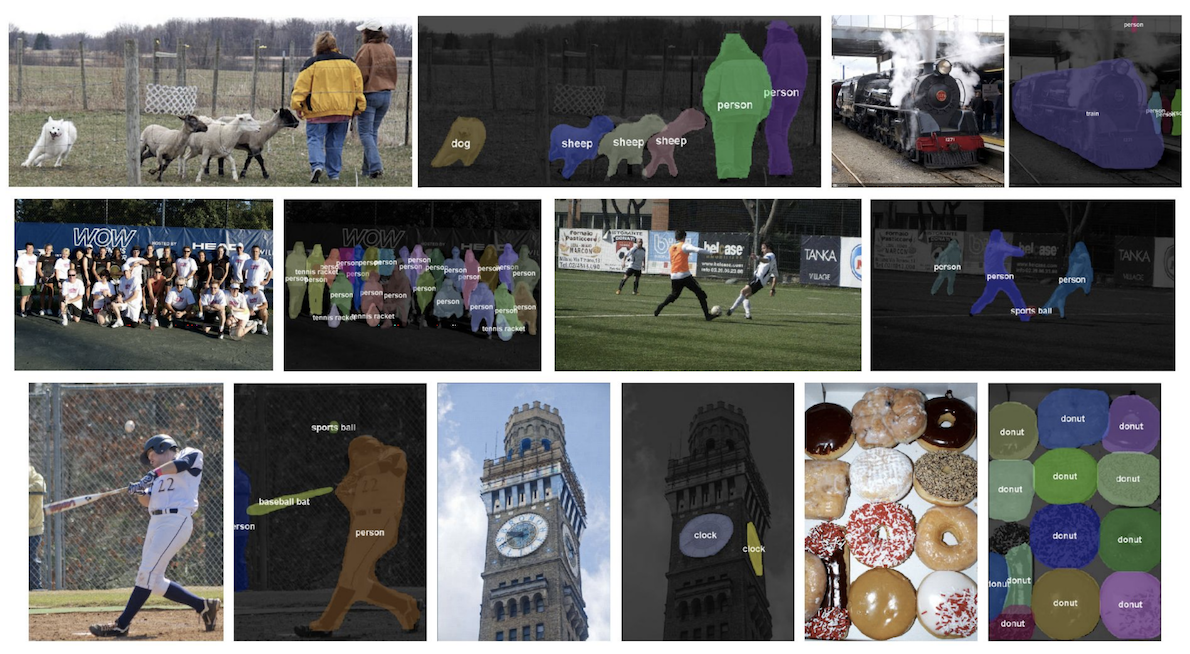
\includegraphics[width=12cm]{segmentation.png}
\centering
\caption{Object segmentation results from \cite{semseg}.}
\end{figure}

\

\subsection{Pose Estimation}

\textit{Pose estimation} involves tracking the skeleton of a human body configuration to understand what humans are doing across a sequence of images; \cite{poseest} uses convolutional neural networks to jointly learn to locate body parts and to then associate them with distinct individuals in an image.

\begin{figure}[h]
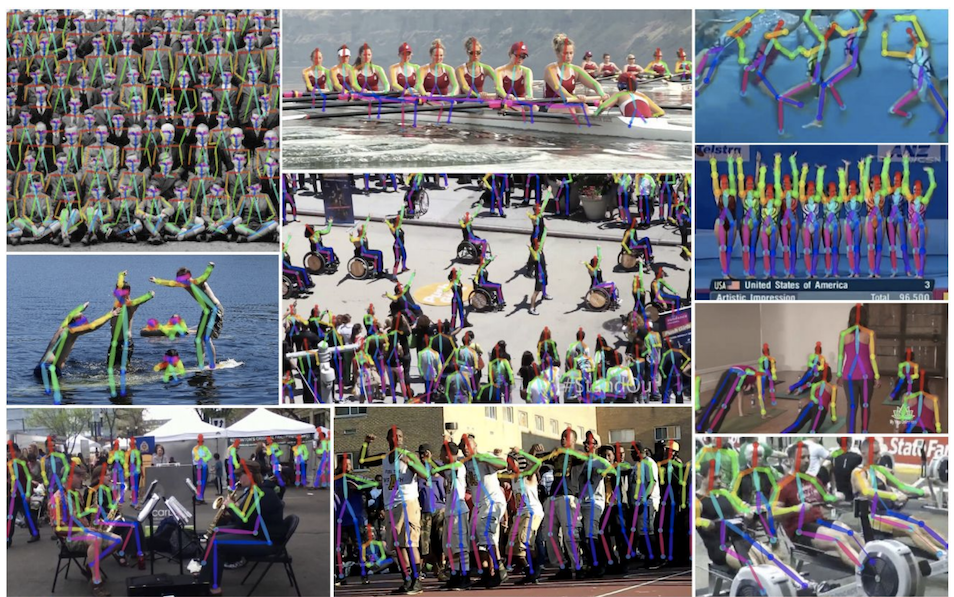
\includegraphics[width=12cm]{poseest.png}
\centering
\caption{Pose estimation results from \cite{poseest}; here, identified human skeletons are labeled with bright colors to indicate pose.}
\end{figure}

\subsection{Image Captioning}

\textit{Image captioning} is just what the name implies\textemdash algorithmically understanding the objects, actions, and relationships in an image to come up with a coherent English description of what that image depicts. Deep learning has demonstrated impressive results for this task: \cite{singlecap} uses a combination of convolutional and recurrent neural networks to label images with a single caption, and \cite{densecap} uses a similar architecture plus an additional neural network layer that is responsible for localizing distinct objects/actions in an image to densely label an image with a caption for each object/action it depicts.

\begin{figure}[h]
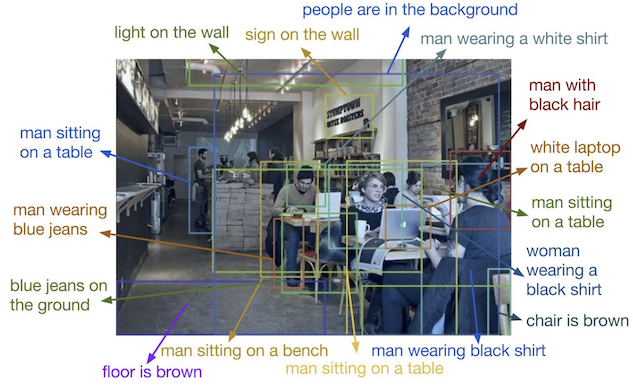
\includegraphics[width=10cm]{densecap.png}
\centering
\caption{Dense image captioning results from  \cite{densecap}.}
\end{figure}

\subsection{Other Computer Vision Tasks}

\textit{Visual question answering} is the task of answering plain-English questions about the objects/actions depicted in input images; for instance, given a picture of a pizza, an algorithm might be expected to answer "How many slices of pizza are there?" or "Is this a vegetarian pizza?". This problem is still considered quite challenging but one method, \cite{vqa}, uses a recurrent neural network-based approach that takes advantage of LSTM (long short-term memory) blocks to answer multiple-choice questions about an image's subjects and their actions.

\textit{Image super-resolution} involves inferring a high-resolution version of a scaled-down input\textemdash this is an inherently difficult task because it involves generating details that you simply don't have to start out with, and making sure that this detail you generate is consistent throughout the image. \cite{superres} uses a relatively recent network architecture called a generative adversarial network to recover realistic textures from downscaled images and managed to produce interpolated results that were closer to the original, high-resolution validation images than any other image super-resolution method.

\subsection{Outside Computer Vision}

Deep learning has also been used to demonstrate extremely impressive results to a variety of tasks outside of computer vision, including machine translation \cite{translation}, text generation \cite{textgen}, speech recognition \cite{sprec}, and speech synthesis \cite{spsyn}.

In addition, "deep reinforcement learning" approaches have demonstrated incredible success for several tasks. Deep reinforcement learning involves learning an optimal control policy (i.e., a series of actions to take given a particular state to reach an end goal) end-to-end through repeated trial-and-error, with the ultimate objective being to directly map state information (e.g., a screenshot of a video game) to the optimal action to take  (e.g., the controller buttons to hit/directional pad inputs to supply). This approach has been used to demonstrate remarkable results for many game-based tasks in particular, including learning how to play  Atari games \cite{atari} and beating the world champion in the strategy board game Go \cite{go}, long considered a benchmark of AI progress.

\section{Motivation}
Most deep learning problems are formulated as supervised learning tasks; data $X$ and labels $y$ are given, and the goal is to learn accurate predicted labels $\hat{y}$. Image classification (in which we want to place an image into one of several pre-specified categories) is a supervised learning task commonly addressed with deep learning approaches. The other approaches to image classification we've covered first extract hand-designed features, then use machine learning approaches (e.g. PCA or KNN) to learn models on this restricted feature set; at test time, we use the classifier output $\hat{y}$ as our predicted classification. Critically, the feature extractor is hand-designed and cannot be optimized during training.
\begin{figure}[h]
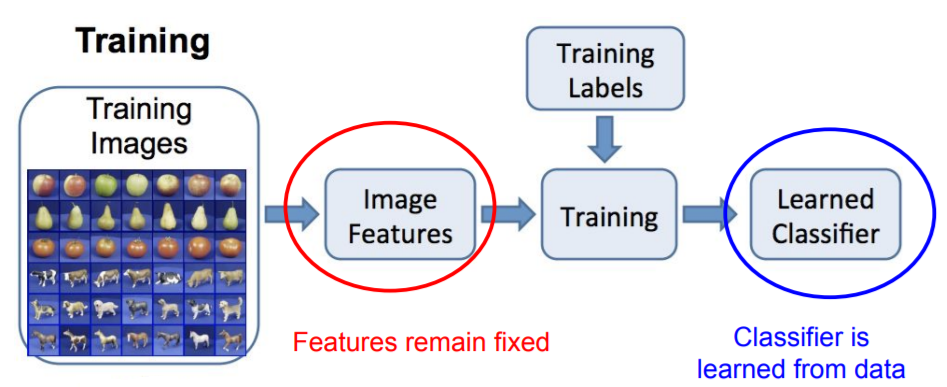
\includegraphics[width=6cm]{Conventional_schematic.png}
\centering
\caption{Image classification with "traditional" computer vision. (CS 131 lecture slide 19-28)}
\end{figure}

Most of the strategies covered in this class focused on reducing images to sets of hand-engineered features. These reduced feature sets encode (some of) the original information in the image and can be used to train classifiers through a variety of machine learning approaches. 

\begin{figure}[h]
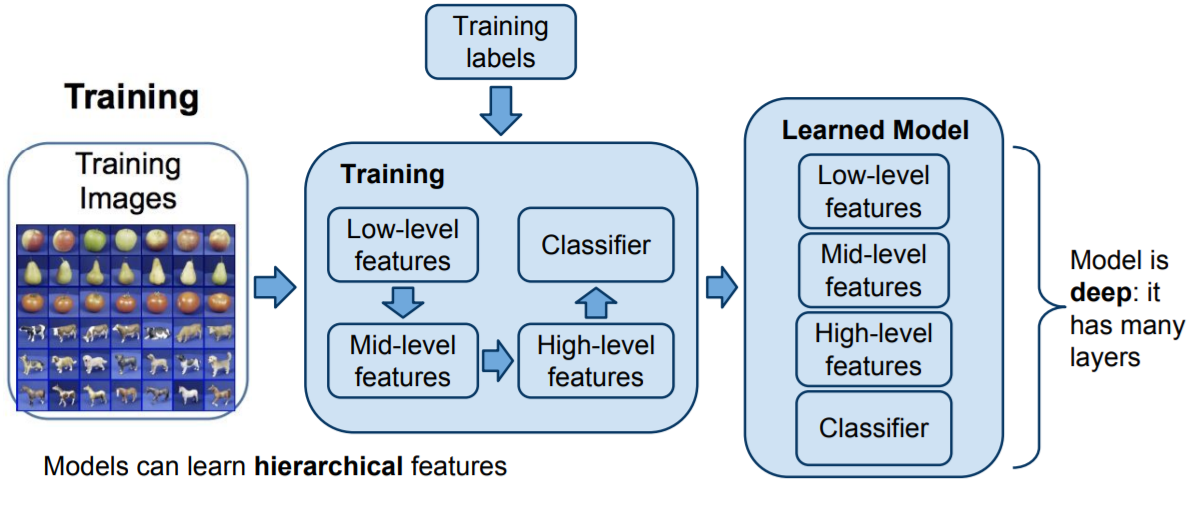
\includegraphics[width=6cm]{DL_schematic.png}
\centering
\caption{Image classification with deep learning. (CS 131 lecture slide 19-32)}
\end{figure}

Deep learning allows us to learn the features \textbf{jointly with the classifier}. This means we can achieve a much better model. Deep learning is motivated by the desire to derive informative features from something closer to first principles, in such a way that the feature extraction and classification modules are optimized together.

\begin{figure}[h]
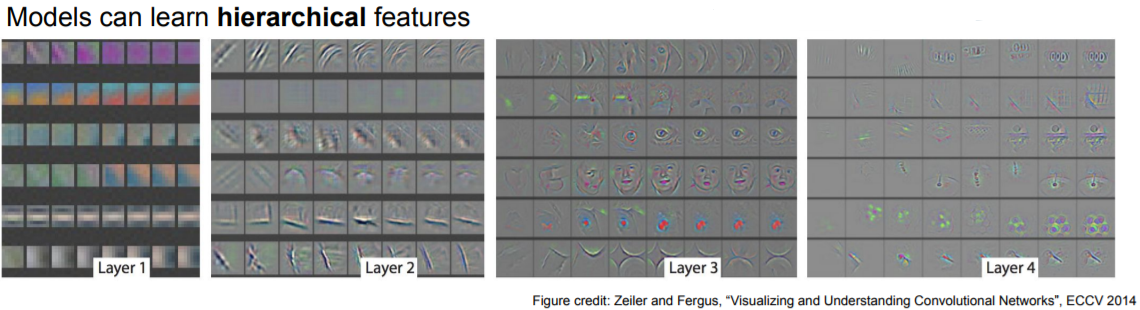
\includegraphics[width=6cm]{Hierarchical_features.png}
\centering
\caption{Hierarchical features emerge in deep learning models. (CS 131 lecture slide 19-33)}
\end{figure}

Deep learning models contain many layers, which learn hierarchical features. Lower layers learn simple features, while higher layers learn combinations of those.
\section{Supervised Learning}

\subsection{Problem Formulation}
Supervised learning is the process of learning a function from labeled training data. Given a set of training examples, the model will adjust its weights so as to minimize the value of its cost function — an expression like the mean squared error that measures how different predicted and actual values are. Oftentimes, this loss function will include a regularization term,R(w), that penalizes large weight values and limits model complexity. The model can then use these calculated weights to predict output labels or values for testing data. The testing error can subsequently be evaluated and used for model performance analysis. 

The following equation provides a general solution to the problem of supervised learning. 

$$W^* = \arg\min_{W} \frac{1}{N} \sum_{i=1}^{N} l(f(x_{i},w),y_{i}) + R(w)$$


\subsection{Linear Regression}
Linear regression is a method of supervised learning where we attempt to model an input vector $x_i\in \mathbb{R}^{D_{in}}$ to an output vector $y_i\in \mathbb{R}^{D_{out}}$. Linear regressions attempts to model this through a simple linear transformation or matrix multiply:

$$f(x, W) = Wx$$

We can pose this as a learning problem where we attempt to learn the weights of $W$ by optimizing the a loss function which combines the euclidean distance $l(\hat{y},y) = \frac{1}{2} ||\hat{y} - y||_2^2$ with a regularizer $R(W)$. Using the frobenius regularizer, we can formally define this optimization problem as follows:

$$W^* = \arg\max_{W} \frac{1}{2N} \sum_{i=1}^{N} ||Wx_i - y||_2^2 + \lambda ||W||_{fro}^2$$

\begin{figure}[h]
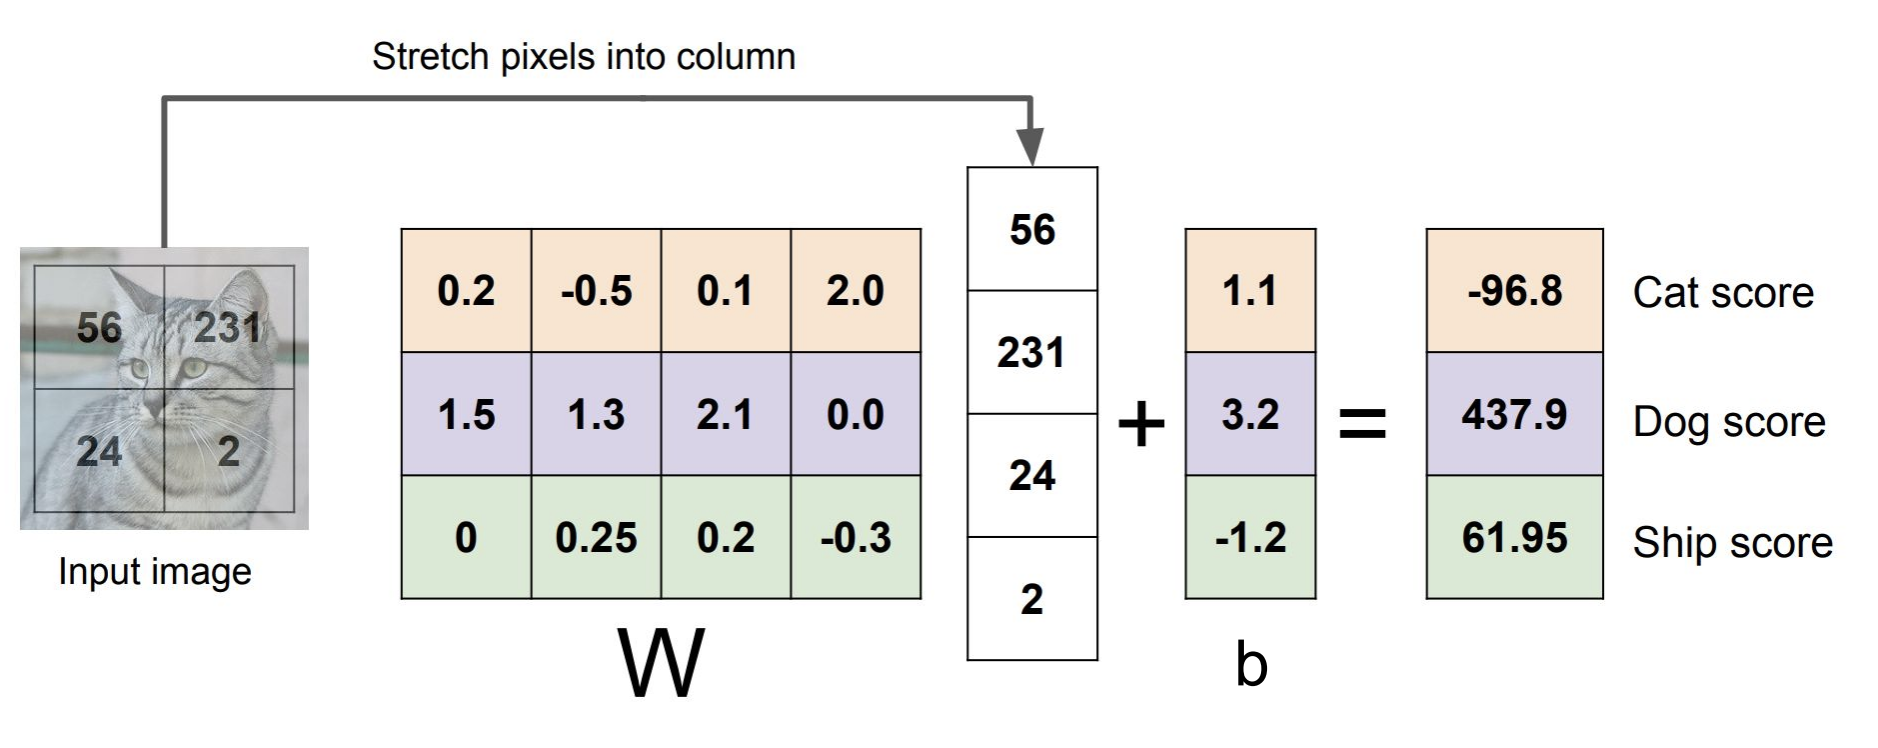
\includegraphics[width=8cm]{Linear_regression.png}
\centering
\caption{An example of a simple linear regression model being used to classify an image. Each row of $W$ represents the weights used to sum the input for each output class. (CS 131 lecture slide 19-42)}
\end{figure}
\subsection{Neural Networks}
In some cases, a simple linear transformation is too simplistic of a function for our purposes and we would like to introduce a more complex model for our supervised learning task. At first, we may be tempted to merely introduce additional matrix multiplies as follows:

$$f(x, W_1, W_2) = W_2W_1x$$

This however, does not actually introduce any additional model complexity since $W_1W_2$ can be written as just one matrix multiply where $W = W_1W_2$, which brings us back to our original linear regression function, $f(x, W) = Wx$. Instead, we need to introduce nonlinearities between each matrix multiply. This produces the following new model where $W_1\in \mathbb{R}^{H \times D_{in}}$ and $W_2\in \mathbb{R}^{D_{out} \times H}$:

$$f(x,W_1,W_2) = W_2(\sigma(W_1x))$$ 

In this model, a matrix multiply $W_1$ is followed by an element-wise non-linearity function $\sigma : \mathbb{R}^H \Rightarrow \mathbb{R}^H$, which is followed again by another $W_2$ matrix multiply. This is an example of a one-layer neural network. The introduction of the non-linearity function, $\sigma$, allows this model to be much more expressive and powerful than a simple linear model.  

Given that the use of the non-linearity function is a large part of what makes neural networks superior to basic linear models, a great deal of research has gone into finding the optimal function for use in these systems. The sigmoid function, defined as $\sigma(x) = \frac{1}{1+e^{-x}}$ has risen to popularity in part because it is continuous and easy to differentiate, while also bounding its inputs. Meanwhile, the rectified linear unit, defined as defined as $\sigma(x) = max(0,x)$ is another example of a popular activation function that has seen superb performance in literature as well as favorable efficiency.

\begin{figure}[h]
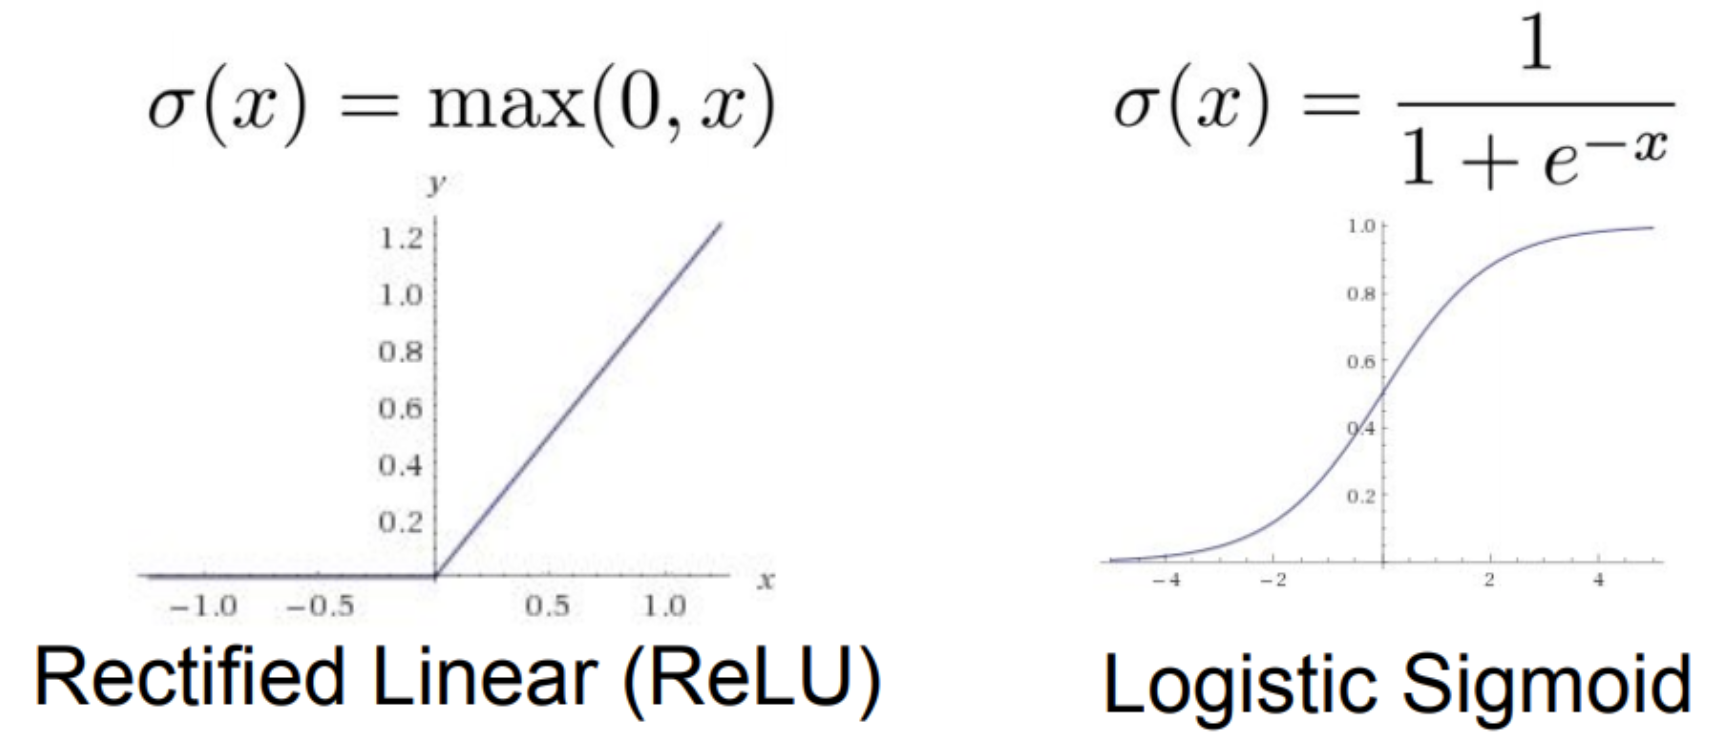
\includegraphics[width=7cm]{activation_functions.png}
\centering
\caption{Depictions of the rectified linear unit and sigmoid activation functions (CS 131 lecture slide 48)}
\end{figure}

The vector produced by each non-linearity (also called the activation function) is called a hidden layer. These types of models can be increased in size to include more matrix multiplies and thus more hidden states. The previous, one-layer neural network can be expanded to a two-layer neural network as follows:

$$f(x,W_1,W_2,W_3) = W_3\sigma(W_2(\sigma(W_1x))$$ 

Given a differentiable loss function (we can use the same one used in linear regression), this new neural network architecture can be optimized using a variety of optimization techniques. As the network is trained, the hidden layers begin to represent "learned features" regarding the input. Importantly, this is one of the primary motivations behind this type of model as it moves away from hand-crafted features.

\begin{figure}[h]
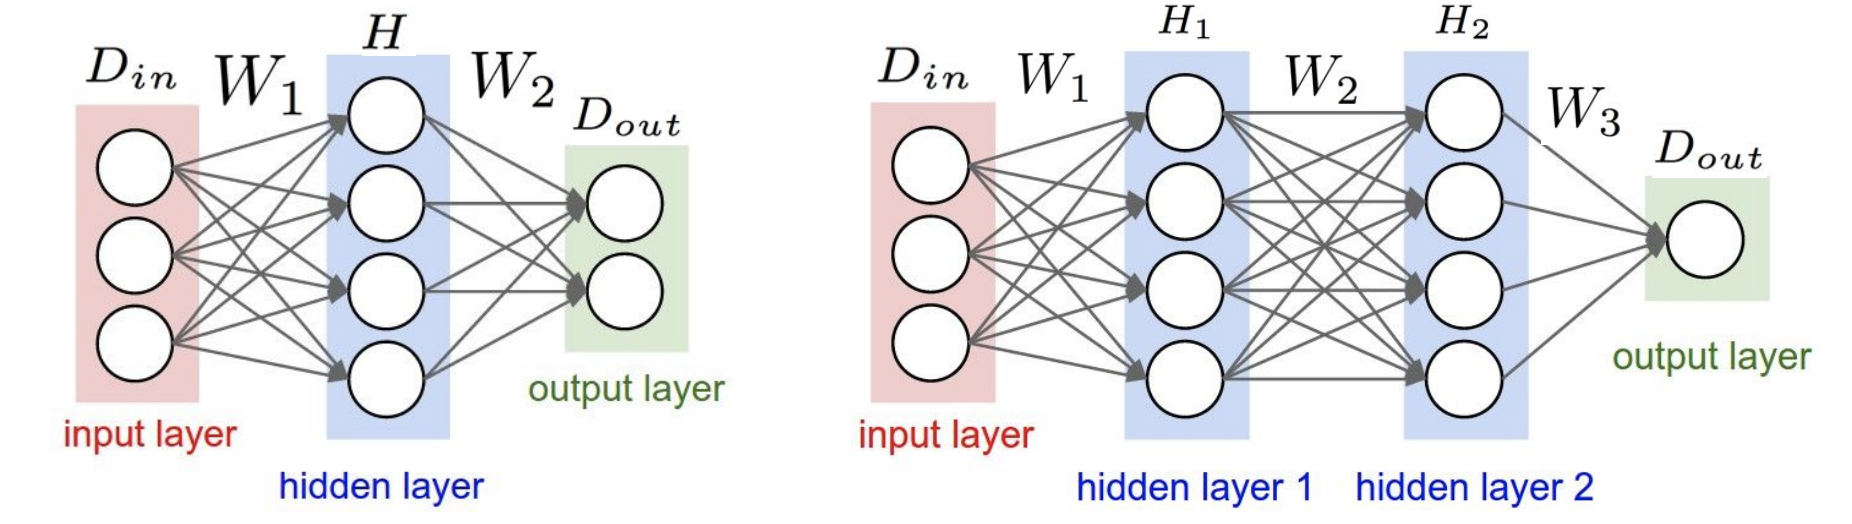
\includegraphics[width=9cm]{neural_network.png}
\centering
\caption{An graphical representation for one-layer and two-layer neural network architectures. (CS 131 lecture slide 19-52)}
\end{figure}

\section{Gradient Descent}
Optimization of weights in a machine learning algorithm is key to building a more robust algorithm with predictive power. As described above, we ultimately want to minimize the following function to help determine the best weights:

$$ g(w) = \frac{1}{N} \sum_{i=1}^{\infty} l(f(x_i, w), y_i) + R(w)$$

One approach to optimize this function is a closed form solution (directly solving through an equation) but this method can be highly expensive. Similarly, random search for the best weights is inefficient especially for high dimensions.

The goal of gradient descent is to efficiently search for optimized parameters that improve the preformance of the model rather than trying to randomly search through weights. Gradient descent works by calculating how the function $g(w)$ changes given small changes in the weight vector $w$. The classic way to determine this change is by calculating the derivative $g'(w)$ assuming w is scalar, but if w is a vector (representing features in multiple dimensions) then we must calculate the gradient of $g(w)$ across each component of $w$

Based on this idea, we can come up with a straightforward algorithm for gradient descent that is useful in deep learning:

\begin{algorithm}[H]
Initialize w randomly \\
 \While{true}{
  read current\;
 Compute gradient $\nabla g(w)$\;
w = w - $\alpha*\nabla g(w)$
 }
\end{algorithm}

With this approach, we can iteratively update the weights of our model and use the learning rate ($\alpha$), which is a hyper-parameter that tells gradient descent how quickly to step in search for a minimum.



\section{Convolutional Neural Networks}
Convolutional neural networks are a very successful and commonly used subset of deep learning models, which adapt the convolutional filters discussed in earlier lectures. Starting from an original image (say, 32x32 with 3 color channels), the image is convolved with multiple filters. (In the example used in class, a 5x5 filter was used, only over the "valid" region of the image - so no overlap with the region outside the image; the output side length is 32-5+1 = 28.) Crucially, the parameters of these filters are optimized jointly via backpropagation - we are no longer limited to hand-chosen features.

\begin{figure}[h]
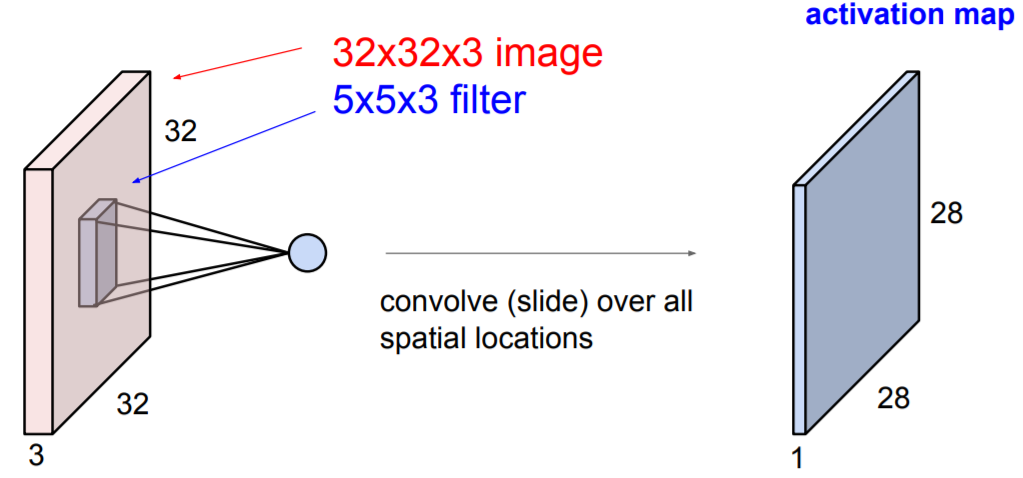
\includegraphics[width=6cm]{Activation_map.png}
\centering
\caption{Extracting an activation map from a raw image in a CNN layer. (CS 131 lecture slide 19-97)}
\end{figure}

 Using convolutions gives us translational invariance - a feature is expected to mean the same thing no matter where in the image it appears. Multiple independent convolutional filters can be passed over the original image, and the outputs stacked to give what is essentially another image with more channels. Nonlinearities are applied as in other deep learning models, and further convolutional layers can be trained on this output to learn higher-level features (combinations of the lower-level features). This allows for the expressive models arising from simple components which are a hallmark of deep learning.
 
\begin{figure}[h]
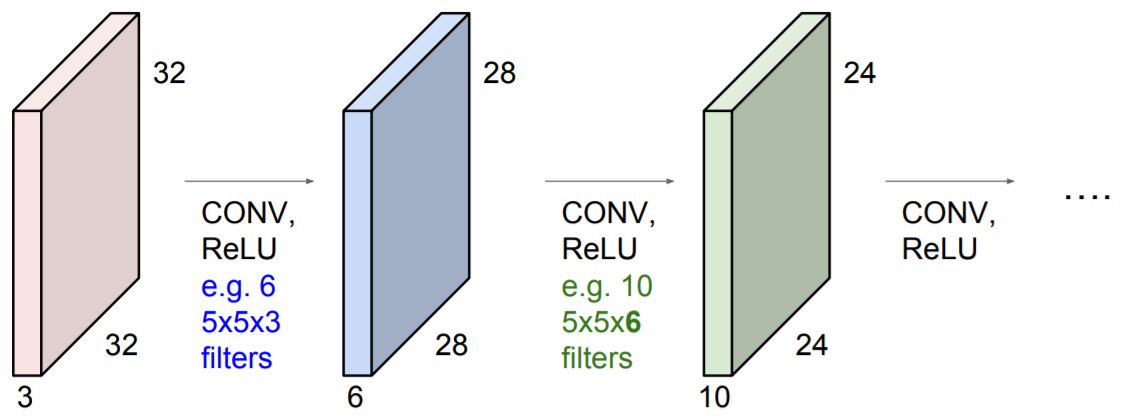
\includegraphics[width=6cm]{CNN_stacking.png}
\centering
\caption{Stacking CNN layers to build a deeper model. (CS 131 lecture slide 19-100)}
\end{figure}



The GoogLeNet case study takes this approach one step further by building "Inception modules" - a particular pattern of layers which are then concatenated. To train this deep net, Szegedy et al. \cite{DBLP:journals/corr/SzegedyLJSRAEVR14} used "auxillary classifiers" to effectively try to predict image class based on only some of the GoogLeNet's layers; in training, a weighted sum of all outputs was used as the loss function.

\begin{figure}[h]
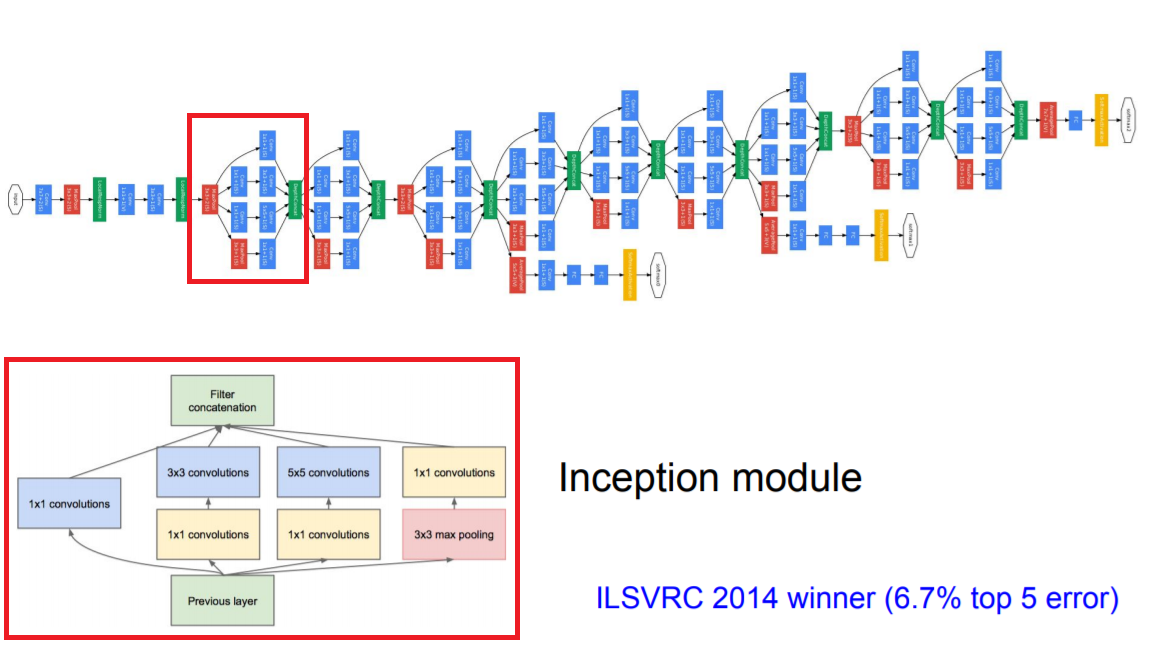
\includegraphics[width=6cm]{Inception.png}
\centering
\caption{GoogLeNet architecture and Inception module. (CS 131 lecture slide 19-101)}
\end{figure}
 
\section{Conclusion}
Deep learning is a relatively recent paradigm in computer vision and related machine learning fields which co-trains feature extractors and classifiers instead of relying on human skill to identify salient features. Deep learning approaches are the state of the art in most computer vision problems today; however, in settings where training examples are expensive or inherently limited, other methods covered in this class can still be very useful, as human intuitions about a problem domain can be used to choose good sets of features.
% References
\small
\bibliographystyle{plain}
\bibliography{bibliography}
\end{document}
